\chapter{Problema 1: Validação de Módulo de Tracking}
\label{chap:val_ids}

\section{Introdução}
\label{chap3:sec:intro}
Durante um processo de \textit{tracking} de qualquer objeto, erros podem acontecer. No caso específico abordado pelo presente projeto, a partir de imagens captadas por painéis de \textit{outdoor}, \textit{bounding boxes} foram colocadas ao redor das pessoas que passavam pelos locais abrangidos. IDs únicos foram igualmente atribuídos, constituindo, em teoria, a ação de \textit{tracking}.

\noindent Assim, o primeiro desafio proposto passou por validar os IDs atribuídos aos diferentes indivíduos, tomando como entrada uma sequência de \textit{patches} e avaliar se diz respeito ao  mesmo indivíduos ou a indivíduos diferentes.

\begin{figure} [h]
  \centering
  \begin{subfigure}{385pt}
    \centering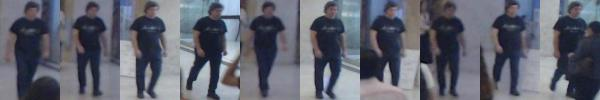
\includegraphics[width=385pt]{capa.jpg}
    \caption{}
  \end{subfigure}
  \begin{subfigure}{385pt}
    \centering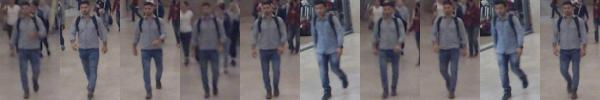
\includegraphics[width=385pt]{capa2.jpg}
    \caption{}
  \end{subfigure}
  \caption{Exemplos de sequências respeitantes a um mesmo indivíduo (a) e a indivíduos diferentes (b).}
  \label{fig:imagem_exemplo}
\end{figure}

\section{Pré-processamento dos dados}
\label{chap3:sec:metodo}
Antes de passarem pela etapa de aprendizagem, os dados foram trabalhados de modo a configurarem entradas válidas na \ac{CNN}. A figura \ref{fig:movimentos} apresenta alguns casos práticos e a figura 3.3 apresenta de forma esquemática as etapas necessárias, sendo expostas com maior detalhe nas secções seguintes. \newline

\begin{figure} [h]
  \centering
  \begin{subfigure}{4cm}
    \centering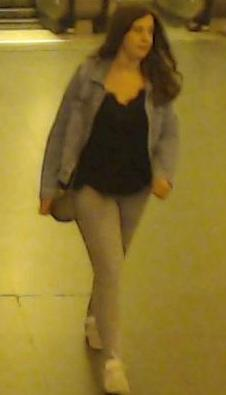
\includegraphics[width=3.5cm]{aproxima.jpg}
    \caption{}
  \end{subfigure}
  \begin{subfigure}{4cm}
    \centering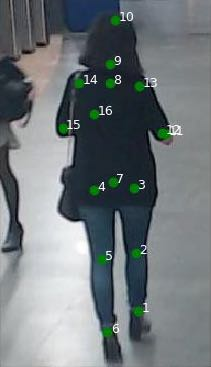
\includegraphics[width=3.5cm]{esqueleto.jpg}
    \caption{}
  \end{subfigure}
  \begin{subfigure}{4cm}
    \centering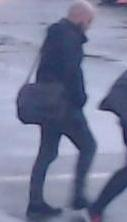
\includegraphics[width=3.5cm]{lateral.jpg}
    \caption{}
  \end{subfigure}
  \caption{3 principais tipos de movimento: aproximação (a), afastamento - com dados de pose - (b) e lateral (c).}
  \label{fig:movimentos}
\end{figure}

\begin{figure}[h]
    \centering
    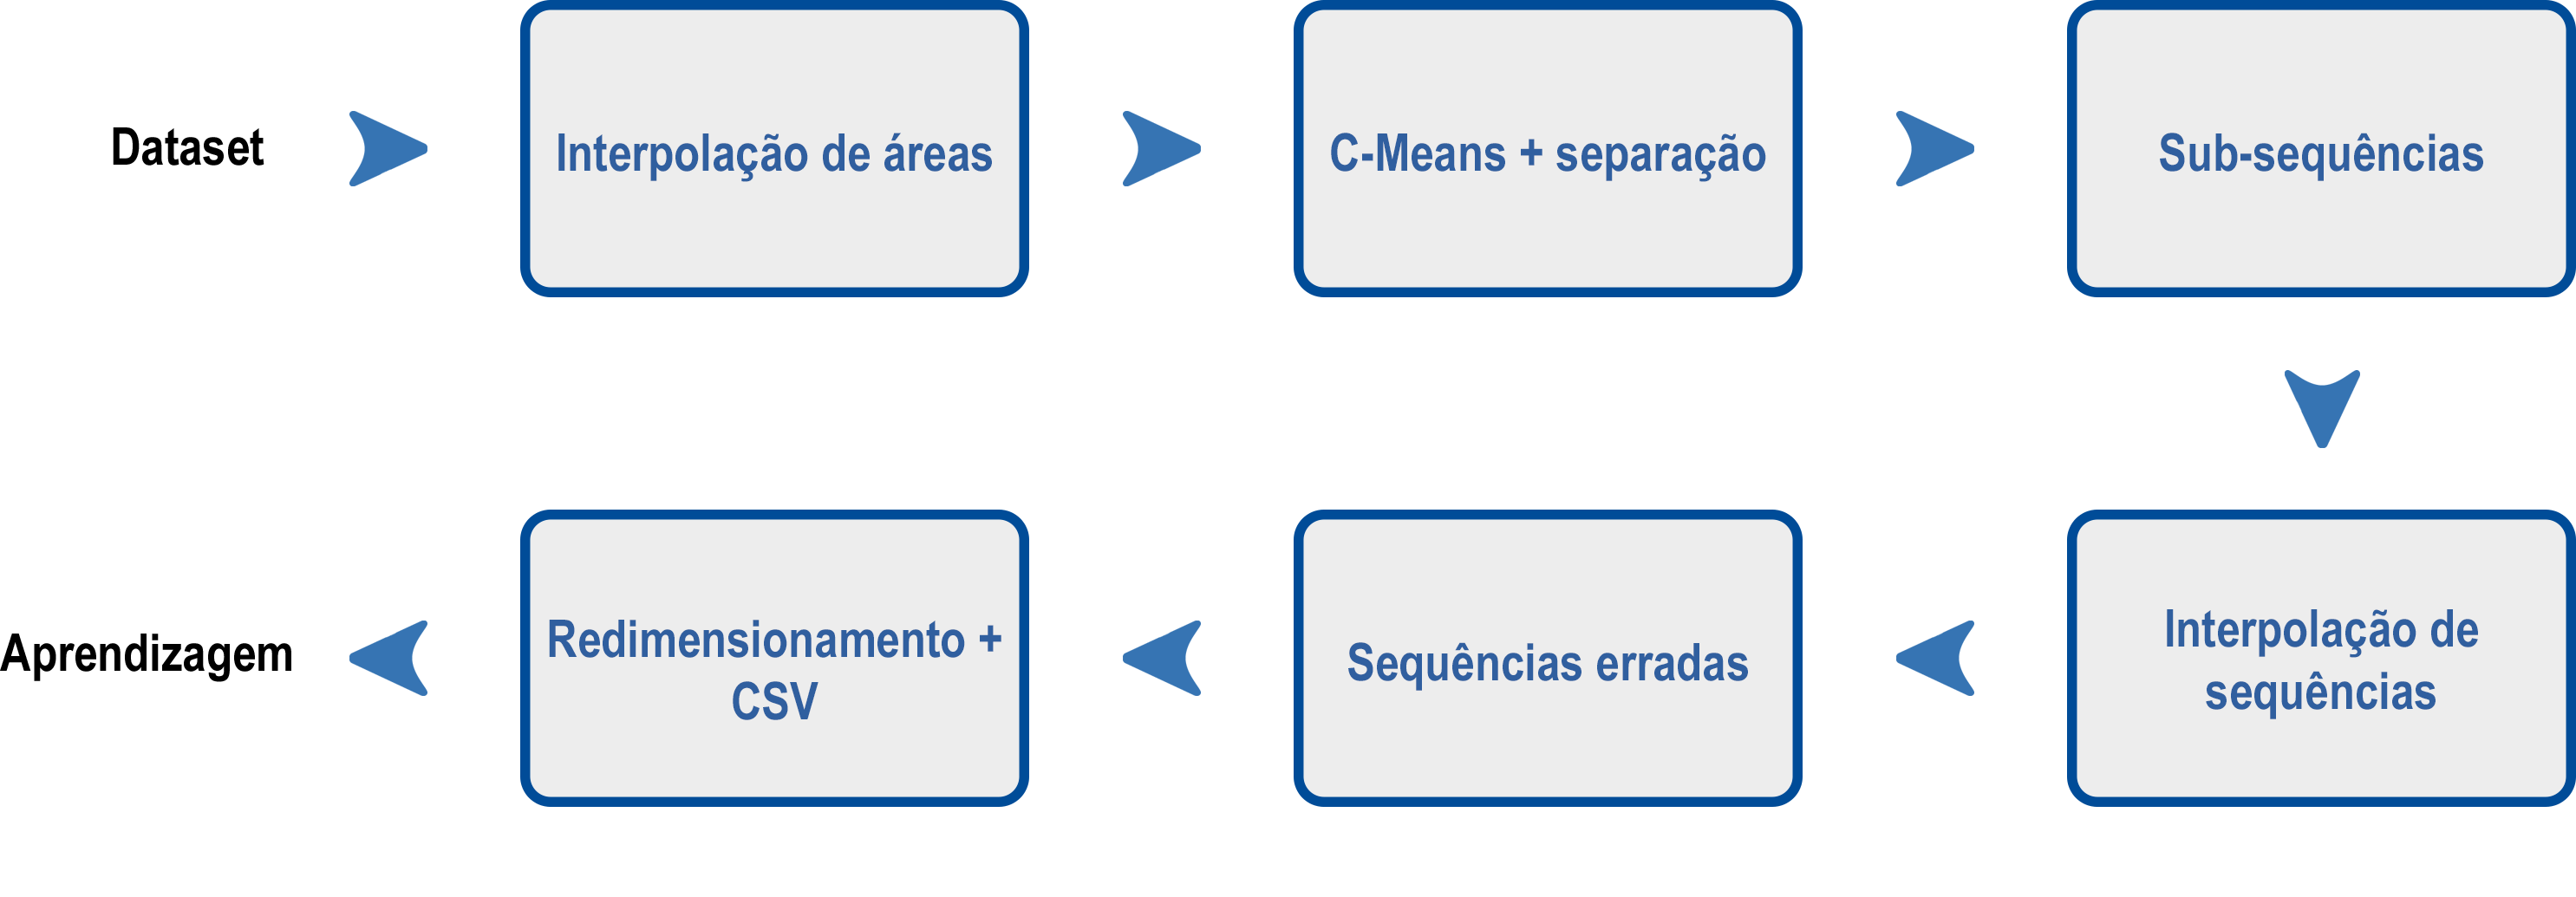
\includegraphics[width=380pt]{pipeline.png}
    \label{fig:pipeline}
    \caption{\textit{Pipeline} de pré-processamento.}
    \end{figure}

\subsection{Interpolação de áreas}
\label{chap3:subsec:areas}
Cada \textit{patch} de cada indivíduo possui, naturalmente, uma altura e uma largura (em píxeis), e, por consequência, uma área. Numa primeira fase é importante discriminar o tipo de movimento de uma pessoa para a geração de instâncias erradas de uma sequência ser possível (mais se acrescenta num próximo ponto). Assim, as áreas são calculadas, normalizadas no intervalo [0,1] e interpoladas (para haver um número constante para todos os indivíduos). 

\noindent Note-se que existe a possibilidade de existirem menos \textit{patches} do que o número definido (25, por exemplo). A solução passou por obter o gráfico do movimento com os dados reais e calcular dados artificiais. A figura 3.4 apresenta um movimento de afastamento expandido.
    
\begin{figure}[h]
\centering
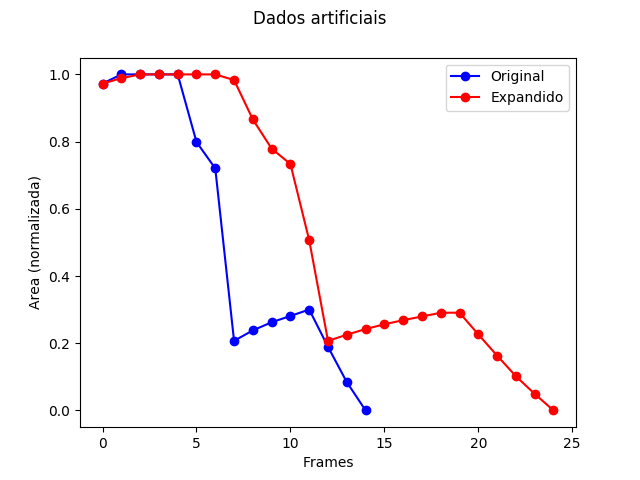
\includegraphics[width=270pt]{interpolada.png}
\label{fig:dados_artificiais_foto}
\caption{Obtenção de mais valores de área.}
\end{figure}

\subsection{Algoritmo C-Means e separação de sequências}
\label{chap3:subsec:cmeans}
O algoritmo C-Means representa uma forma de \textit{fuzzy clustering}, na qual os elementos são agrupados em \textit{clusters} de acordo com as suas caraterísticas. Elementos de um mesmo \textit{cluster} tendem a ser o mais semelhantes possível, enquanto que se procura maximizar a diferença entre elementos de \textit{clusters} distintos. De notar que um elemento pode pertencer a um ou mais \textit{clusters}.

\noindent A noção de pertença (ou \textit{membership}) é basilar neste algoritmo. Pontos/elementos mais afastado do centro de um \textit{cluster} têm graus de \textit{membership} mais baixos; em sentido inverso, quanto mais perto do centro, maior é o grau. 

\noindent O propósito deste algoritmo passa por minimizar a seguinte função objetivo:

\begin{equation}
 \operatorname*{argmin}_C\sum_{i=1}^{C}\sum_{k=1}^{N}u_{ik}^m||x_k-c_i||^2.
 \label{eq:eq1}
\end{equation}

\noindent Na fórmula \ref{eq:eq1} o parâmetro \emph{C} representa o número de grupos a considerar, \emph{N} o número de pontos/elementos, \emph{m} o \textit{fuzzifier} (tem efeito sobre a performance do algoritmo) e \emph{$u_{ik}$} o coeficiente de \textit{membership} (aparece multiplicado pela distância de cada ponto - \emph{$x_k$} - a um dado centro - \emph{$c_i$}). Por sua vez, os coeficientes de \textit{membership} e os centros possuem as seguintes fórmulas, respetivamente:

\begin{equation}
u_{ik} = \frac{1}{\sum_{j=1}^{C}{\left( \frac{||x_k-c_i||^2}{||x_k-c_j||^2} \right)}^{\left( \frac{1}{m-1}\right)}}.
 \label{eq:eq2}
\end{equation}

\begin{equation}
c_{i} = \frac{\sum_{k=1}^{N}{u_{ik}^{m}x_k}}{\sum_{k=1}^{N}{u_{ik}^{m}}}.
 \label{eq:eq3}
\end{equation}

\noindent A execução do algoritmo baseia-se em em várias iterações com vista a minimizar a função objetivo (\ref{eq:eq1}) e cujo critério de paragem é, normalmente, atingido quando a diferença entre os coeficientes obtidos em iterações sucessivas for menor que um dado parâmetro (\emph{$\epsilon$}).

\noindent O C-Means foi aplicado sobre os valores normalizados e interpolados das áreas, para obter os dois padrões dominantes (essencialmente, os movimentos de afastamento e aproximação) - figura 3.5. Os valores de cada indivíduo são depois comparados com cada padrão, determinando com qual dos dois existe maior semelhança. Adicionalmente, os dados de pose (fornecidos com este \textit{dataset}) são também usados para determinar o tipo de movimento, nomeadamente através da posição dos ombros entre si.

\begin{figure}[h]
\centering
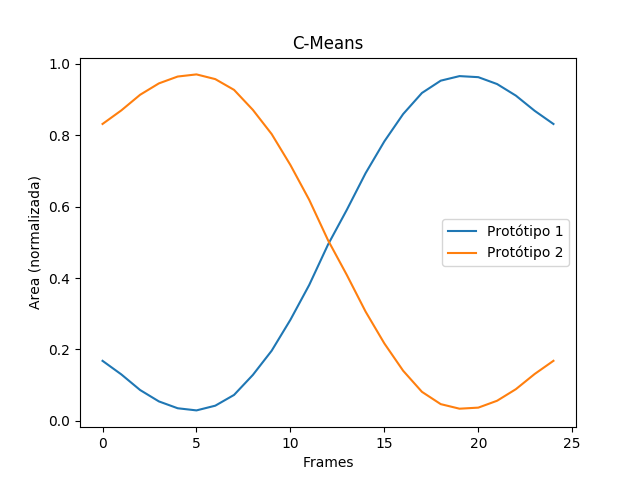
\includegraphics[width=220pt]{c-means_25.png}
\label{fig:c_means}
\caption{Padrões extraídos com o C-Means.}
\end{figure}

\subsection{Geração de sub-sequências}
\label{chap3:subsec:sub}
De modo a aumentar a quantidade de dados disponíveis, foram geradas sub-sequências a partir das sequências separadas anteriormente. Uma sub-sequência é simplesmente uma variação da original. Por exemplo, a partir de uma sequência com 20 \textit{patches}, pode-se obter uma variação que contém as imagens no intervalo [1,15].

\subsection{Interpolação de sequências}
\label{chap3:subsec:interpolar_seq}
Dado que nem todos os indivíduos têm o mesmo número de \textit{patches}, definiu-se um tamanho constante para as sequências dadas à \ac{CNN}. Todas as sequências que não cumprirem com este requisito são descartadas. Por outro lado, se uma sequência tiver mais imagens que as necessárias, será interpolada para atingir o tamanho desejado.

\subsection{Geração de sequências erradas}
\label{chap3:subsec:erradas}
Para cada sequência foi gerada uma instância errada. Se o tamanho definido para as sequências for "x", "x-1" ou "x-2" imagens mantêm-se na sequência errada. No caso de só se trocar uma imagem, a que não se manteve é substituída por uma de outra sequência (efetivamente outro indivíduo do mesmo conjunto - treino, validacao ou teste - com um tipo de movimento semelhante). O processo é semelhante se se trocarem duas imagens. Esta troca pode ser feita de forma aleatória ou de forma mais informada (e difícil de detetar):

\begin{enumerate}
    \item \textbf{Troca aleatória:} É sorteado um indivíduo do mesmo conjunto. Uma ou duas \textit{patches} são colocadas na instância errada da sequência original, completando a errada.
    \item \textbf{Troca informada:} É escolhido o indivíduo mais aproximado ao da sequência original, sendo que todos os indivíduos candidatos são classificados num total de 100 pontos - 80 dizem respeito à cor da roupa e 20 às \textit{soft biometrics} dos indivíduos, como o tipo e cor de cabelo, a fisionomia do corpo, entre outros. \newline \noindent O indivíduo com menor distância em termos de cor em cada um dos 16 pontos de esqueleto recebe 80 pontos; o segundo melhor recebe um pouco menos e assim sucessivamente (com os extras o processo é análogo). Note-se que a distância de cor para cada ponto de esqueleto é a distância entre as três cores RGB dos pontos.\newline \noindent Estando escolhido o indivíduo com melhor classificação, são colocadas as \textit{patches} na instância errada a ser construída num dado momento. 
\end{enumerate}{}

\begin{figure} [h]
  \centering
  \begin{subfigure}{13.5cm}
    \centering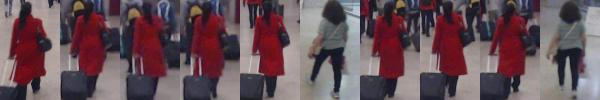
\includegraphics[width=13.5cm]{troca_aleatoria.jpg}
    \caption{}
  \end{subfigure}
  \begin{subfigure}{13.5cm}
    \centering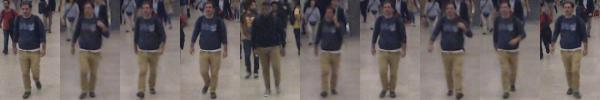
\includegraphics[width=13.5cm]{troca_boa.jpg}
    \caption{}
  \end{subfigure}
  \caption{Troca aleatória (a) e informada (b).}
  \label{fig:trocas}
\end{figure}

\subsection{Redimensionamento das sequências e ficheiro CSV}
\label{chap3:subsec:redim}
A \ac{CNN} usada requer que todas as imagens de entrada tenham um tamanho constante. Assim esta etapa passa por redimensionar todas as \textit{patches} para um tamanho único (definiu-se 60x100).\newline
\noindent Por último, é gerado um ficheiro CSV em que cada linha representa uma sequência, sendo marcadas como destinadas a treino, validação ou teste, bem como se são certas (sempre o mesmo indivíduo) ou erradas. \newline
\noindent

\section{Fase de aprendizagem}
\label{chap3:sec:aprendizagem}
O processo de treino da \ac{CNN} possui variabilidade, nomeadamente na geração de instâncias erradas para cada sequência válida. Tais variações têm impacto na performance sobre os conjuntos de treino, validação e, sobretudo, de teste.\newline
\noindent A figura \ref{fig:graficos} apresenta várias instâncias de aprendizagem, cujas diferenças residem na variablidade acima mencionada.

\noindent Na figura \ref{fig:graficos} estão as seguintes configurações:
\begin{enumerate}[(a)]
    \item Treino e validação informados + teste informado.
    \item Treino e validação informados + teste aleatório.
    \item Treino e validação aleatórios + teste informado.
    \item Treino e validação aleatórios + teste aleatório.
\end{enumerate}{}

\begin{figure} [h]
  \centering
  \begin{subfigure}{6.8cm}
    \centering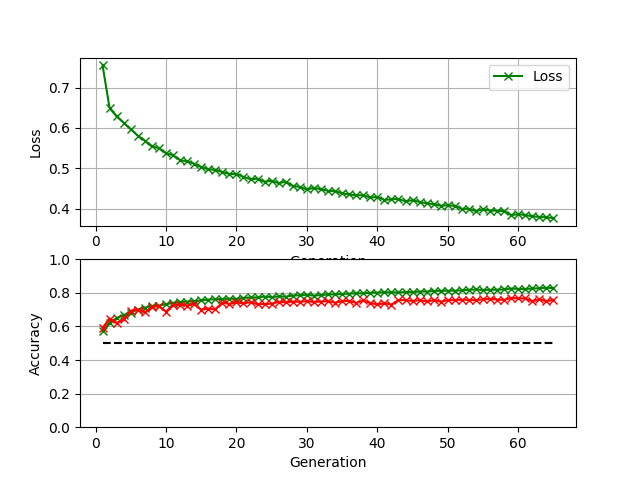
\includegraphics[width=6.8cm]{bom_bom.png}
    \caption{}
  \end{subfigure}
  \begin{subfigure}{6.8cm}
    \centering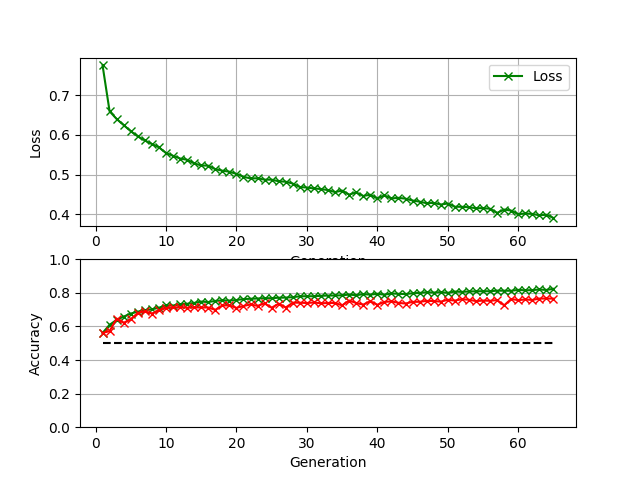
\includegraphics[width=6.8cm]{bom_mau.png}
    \caption{}
  \end{subfigure}
  \begin{subfigure}{6.8cm}
    \centering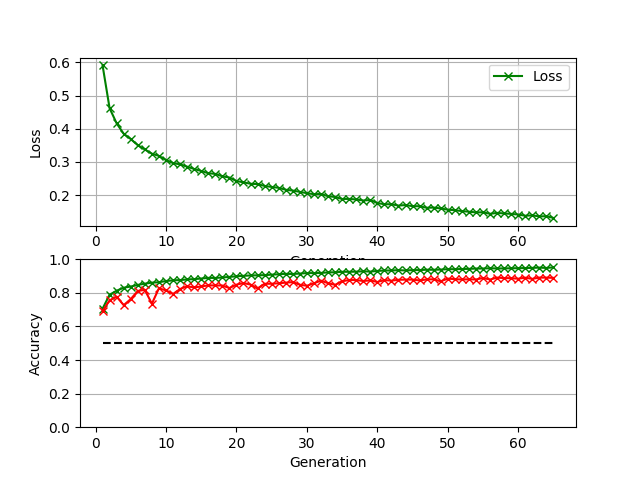
\includegraphics[width=6.8cm]{mau_bom.png}
    \caption{}
  \end{subfigure}
  \begin{subfigure}{6.8cm}
    \centering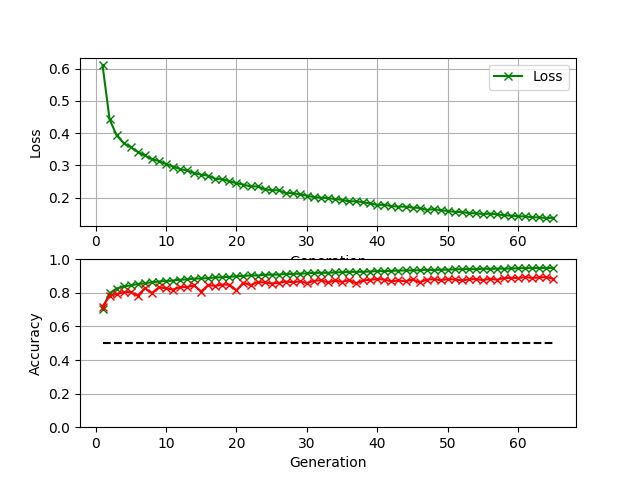
\includegraphics[width=6.8cm]{mau_mau.png}
    \caption{}
  \end{subfigure}
  \caption{Resultados da aprendizagem com 4 configurações diferentes.}
  \label{fig:graficos}
\end{figure}

\begin{table} [!htbp]
\centering
\begin{tabular}{|l|r|r|}
\hline
\textbf{Configuração} & \textbf{Sequências} & \textbf{Acerto}\\
\hline
\hline
Treino e validação informados + teste informado & $\sim62000$ & 78\% \\
\hline
Treino e validação informados + teste aleatório & $\sim63000$ & 84\% \\
\hline
Treino e validação aleatórios + teste informado & $\sim112000$ & 78\% \\
\hline
Treino e validação aleatórios + teste aleatório & $\sim111000$ & 90\% \\
\hline
\end{tabular}
\caption{Taxa de acerto sobre diferentes configurações.}
\label{tab:resultados}
\end{table}

\noindent A tabela \ref{tab:resultados} mostra que se a rede for treinada com um conjunto fácil, existe uma diferença mais significativa entre a performance com dados de teste mais fáceis e mais difíceis (de quase 90\% passa para 78\%). Em contraste, com um treino mais difícil a diferença revela-se muito menor (de quase 84\% para 78\%).


\noindent Note-se que as configurações c) e d) têm mais dados de entrada devido ao facto de que para construir as instâncias negativas de forma informada são usados os dados de pose, sendo que nem todas as imagens os têm.

\section{Discussão e Resultados}
\label{chap3:sec:final}
Uma análise às sequências analisadas pela rede revela alguns casos típicos de falha: uma troca feita na sequência e que a rede não foi capaz de detetar; uma sequência certa mas que contém uma ou mais \textit{patches} com certo ruído (partes de outras pessoas) ou uma sequência com muita interferência (figura \ref{fig:falha}).

\begin{figure} [h]
  \centering
  \begin{subfigure}{13.5cm}
    \centering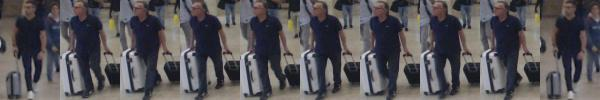
\includegraphics[width=13.5cm]{erro_troca_boa.jpg}
    \caption{}
  \end{subfigure}
  \begin{subfigure}{13.5cm}
    \centering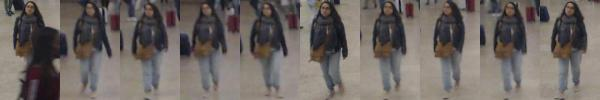
\includegraphics[width=13.5cm]{erro_peq_ruido.jpg}
    \caption{}
  \end{subfigure}
  \begin{subfigure}{13.5cm}
    \centering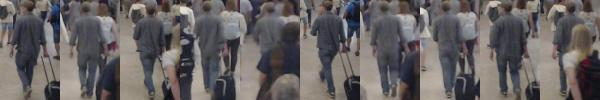
\includegraphics[width=13.5cm]{erro_grande_ruido.jpg}
    \caption{}
  \end{subfigure}
  \caption{Casos típicos de falha.}
  \label{fig:falha}
\end{figure}

\noindent O programa desenvolvido tem como objetivo tomar como entrada uma sequência de tamanho e dimensões iguais aos usados na aprendizagem, e devolver uma simples frase, consoante a sequência diz respeito ao mesmo indivíduo ou a indivíduos diferentes.\newline
\noindent Para testar a solução desenvolvida foram separadas 50 sequências (nunca vistas pela rede) recolhidas de diferentes painéis e em condições de luminosidade diversas, sendo 25 positivas e 25 negativas.\newline
\noindent A taxa de acerto foi de cerca de 52\% usando tanto o modelo treinado com os conjuntos de treino, validação e teste construídos usando a troca informada como usando a troca aleatória. Os parâmetros usados estão descritos na seguinte tabela:

\begin{table}[H]
\centering
\begin{tabular}{|l|r|}
\hline
\textbf{Parâmetro} & \textbf{Valor}\\
\hline
\hline
Épocas & 65  \\
\hline
Taxa de aprendizagem & 0.001  \\
\hline
Probabilidade de \textit{dropout} & 1.0  \\
\hline
Tamanho de \textit{batch} & 100  \\
\hline
Sequências & $\sim75000$  \\
\hline
\hline
\textbf{Acerto (conj. teste)} & \textbf{52\%}\\
\hline
\end{tabular}
\caption{Parâmetros base.}
\label{tab:base}
\end{table}

\noindent Alguns parâmetros foram alterados com vista a avaliar o impacto na performance do sistema. O conjunto de teste usado foi formado pelas 100 sequências separadas (também usadas na performance base, anteriormente descrita). As tabelas seguintes apresentam os parâmetros alterados:

\begin{table}[H]
\centering
\begin{tabular}{|l|r|}
\hline
\textbf{Parâmetro} & \textbf{Valor}\\
\hline
\hline
Épocas & 65  \\
\hline
\textbf{Taxa de aprendizagem} & \textbf{0.0001}  \\
\hline
Probabilidade de \textit{dropout} & 1.0  \\
\hline
Tamanho de \textit{batch} & 100  \\
\hline
Sequências & $\sim75000$  \\
\hline
\hline
\textbf{Acerto (conj. teste)} & \textbf{51\%}\\
\hline
\end{tabular}
\caption{Mudança na taxa de aprendizagem.}
\label{tab:learning_rate}
\end{table}

\begin{table}[H]
\centering
\begin{tabular}{|l|r|}
\hline
\textbf{Parâmetro} & \textbf{Valor}\\
\hline
\hline
Épocas & 65  \\
\hline
Taxa de aprendizagem & 0.001  \\
\hline
\textbf{Probabilidade de \textit{dropout}} & \textbf{0.65}  \\
\hline
Tamanho de \textit{batch} & 100  \\
\hline
Sequências & $\sim75000$  \\
\hline
\hline
\textbf{Acerto (conj. teste)} & \textbf{56\%}\\
\hline
\end{tabular}
\caption{Mudança na probabilidade de \textit{dropout}.}
\label{tab:dropout}
\end{table}

\begin{table}[H]
\centering
\begin{tabular}{|l|r|}
\hline
\textbf{Parâmetro} & \textbf{Valor}\\
\hline
\hline
Épocas & 65  \\
\hline
Taxa de aprendizagem & 0.001  \\
\hline
Probabilidade de \textit{dropout} & 1.0  \\
\hline
\textbf{Tamanho de \textit{batch}} & \textbf{150}  \\
\hline
Sequências & $\sim75000$  \\
\hline
\hline
\textbf{Acerto (conj. teste)} & \textbf{54\%}\\
\hline
\end{tabular}
\caption{Mudança no tamanho de \textit{batch}.}
\label{tab:size}
\end{table}

\noindent Neste caso específico e dados os testes efetuados, o parâmetros que potencialmente afeta mais a performance da rede é a probabilidade de \textit{dropout}.